\documentclass[main.tex]{subfiles}
\begin{document}

\section{Sheet 7}

\subsection{Photons travelling in the Schwarzschild metric}

\subsubsection{A different proof for the conservation of the component of the velocity of a geodesic along a Killing vector field}

Here I present a different proof to what was done in the lectures for the fact that the component of the 4-velocity along the Killing vector field is conserved. 
If the metric does not depend on the coordinate \(\widetilde{\alpha }\), then \(\partial_{\widetilde{\alpha }} g_{\mu \nu } = 0\). So, let us differentiate covariantly the vector \(\xi_{\mu } = g_{\mu \nu } \delta^{\nu}_{\widetilde{\alpha }}\).
It will be apparent later that differentiating the lower-index vector field gives us the interesting property.
We get 
%
\begin{align}
  \nabla_{\mu } \xi_{\nu } =
  g_{\nu \sigma } \nabla_{\mu } \xi^{\sigma }
  =  g_{\nu \sigma }
  \qty(\cancelto{}{\partial_{\mu } \xi^{\sigma }} + \Gamma^{\sigma }_{\mu \rho } \xi^{\rho })
  = \Gamma_{\nu \mu \widetilde{\alpha }}
\,,
\end{align}
%
since the only component which survives the contraction with \(\xi \) is the one along \(\widetilde{\alpha} \); also, we lowered an index of the Christoffel symbols with the metric. 

The explicit expression for the lower indices Christoffel symbols is 
%
\begin{align}
  \Gamma_{\nu \mu \widetilde{\alpha }}
  = \frac{1}{2} \qty(\cancelto{}{g_{\mu \nu , \widetilde{\alpha }}} +
  g_{\mu \widetilde{\alpha }, \nu }
  - g_{\mu \widetilde{\alpha }, \nu })
\,,
\end{align}
%
since by hypothesis any derivative of the metric along \(\widetilde{\alpha}\) is zero. So, we can directly see that the object \(\nabla_{\mu } \xi_{\nu }\) is antisymmetric in its indices: this can be written as 
%
\begin{align}
  \nabla_{(\mu } \xi_{\nu )} = 0
\,,
\end{align}
%
and is called \emph{Killing's equation}. We have shown that is equivalent to the metric not depending on the coordinate \(x^{\widetilde{\alpha}}\).

Now, we can quickly prove the conservation a component of the 4-velocity of a geodesic along the Killing vector field: we just need to differentiate \(u^{\mu } \xi_{\mu }\) with respect to the arc parameter. 
Recall that geodesics are defined by the equation 
%
\begin{align}
 a^{\mu } =  \dv[]{}{s} u^{\mu } = u^{\nu } \nabla_{\nu } u^{\mu } = 0 
\,.
\end{align}
%

We find 
%
\begin{align}
  u^{\nu }\nabla_{\nu }\qty(u^{\mu } \xi_{\mu })
  = u^{\nu } u^{\mu } \nabla_{\nu } \xi_{\mu } + \xi_{\mu } u^{\nu } \nabla_{\nu } u^{\mu } = 0
\,,
\end{align}
%
where both terms are zero: the first because it is the contraction of an antisymmetric object with a symmetric one, and the second one because of the geodesic equation. 

\subsubsection{Conserved quantities in Schwarzschild motion}

The Schwarzschild metric is given by 
%
\begin{align}
  g_{\mu \nu } = \left[\begin{array}{cccc}
  -(1-\frac{2GM}{r}) & 0 & 0 & 0 \\ 
  0 & (1-\frac{2GM}{r})^{-1} & 0 & 0 \\ 
  0 & 0 & r^2 & 0 \\ 
  0 & 0 & 0 & r^2 \sin^2\theta 
  \end{array}\right]
\,
\end{align}
%
in the coordinates \((t, r, \theta , \varphi )\). The vector fields \(\xi_{(t)}^{\mu } = (1, \vec{0})\) and \(\xi_{(\varphi )}^{\mu } = (0,0,0,1)\) in these coordinates are Killing vector fields, since the metric does not depend on \(t\) or \(\varphi \). 

So, the following quantities are conserved in geodesic motion parametrized as \(x^{\mu }(\lambda )\): \footnote{There is a typo in the exercise sheet: a \(G\) is missing in the definition of \(e\).}
%
\begin{align}
  e = -u^{\mu } g_{\mu \nu } \xi^{\nu }_{(t)}
  = -u^{t} g_{tt } \times 1
  = \dv{t}{\lambda } \qty(1 - \frac{2GM}{r})
\,
\end{align}
%
and 
%
\begin{align}
  l = u^{\mu } g_{\mu \nu } \xi^{\nu }_{(\varphi )}
  = u^{\varphi } g_{\varphi \varphi } \times 1
  = \dv{\varphi }{\lambda } r^2 \sin^2\theta 
\,,
\end{align}
%
which for motion on the \(xy\) plane, for which \(\theta = \pi /2\), reduces to \(l = r^2 \dv*{\varphi }{\lambda }\).

\subsubsection{Photons escaping a black hole}

The equation of motion can be derived from the normalization of the photon's four velocity: The equation \(u^{ \mu } u_{\mu }= 0 \) can be  written as 
%
\begin{align}
    \qty(\dv{t}{\lambda })^2 g_{tt} +
    \qty(\dv{r}{\lambda })^2 g_{rr} +
    \qty(\dv{\theta }{\lambda })^2 g_{\theta \theta } +
    \qty(\dv{\varphi }{\lambda })^2 g_{\varphi \varphi } = 0
\,,
\end{align}
%
but the term \(\dv*{\theta }{\lambda }\) is zero if we assume the motion to be in the \(xy \) plane, while the velocity components along \(t\) and \(\varphi \) can be written in terms of the integrals of motion: \(\dv*{t}{\lambda } = e \qty(1 - 2GM/r)^{-1}\) and \(\dv*{\varphi }{\lambda } = l r^{-2}\). So, we find 
%
\begin{align}
  - \qty(1 - \frac{2GM}{r})^{-2+1} e^2 + \qty(1 - \frac{2GM}{r})^{-1} \qty(\dv{r}{\lambda })^2 + l^2 r^{-4} r^2 = 0
\,,
\end{align}
%
we divide through by \(-g_{tt}\) and find: 
%
\begin{align}
    -e^2 + \qty(\dv{r}{\lambda })^2+ \frac{l^2}{r^2} \qty(1 - \frac{2GM}{r}) = 0
    \,,
\end{align}
%
or, dividing through by \(l\):
%
\begin{align}
    -\frac{e^2}{l^2} + \frac{1}{l^2}\qty(\dv{r}{\lambda })^2+ \frac{1}{r^2} - \frac{2GM}{r^3} = 0
\,.
\end{align}

We can give names to the terms in this equation: we call 
%
\begin{align}
  V _{\text{eff}} (r) \equiv \frac{1}{r^2} - \frac{2GM}{r^3}
\,
\end{align}
%
the \emph{effective potential}, and 
%
\begin{align}
  b^2 = \frac{l^2}{e^2}
\,
\end{align}
%
the \emph{impact parameter} (unjustified for now). Then, the equation is in the form 
%
\begin{align}
  \frac{\dot{r}^2}{l^2}  + V _{\text{eff}} (r) = \frac{1}{b^2}
\,,
\end{align}
%
where we denoted derivation with respect to \(\lambda \) with a dot. 
So, we can study the motion of the photon as if it were 1-dimensional. 

To study the problem, it is convenient to use the rescaled adimensional radial coordinate \(R = r / 2GM\). In this variable, the effective potential (which I will denote as just \(V\) hereafter) looks like: 
%
\begin{align}
  V (R) = (2GM)^{-2} \qty(R^{-2} - R^{-3})
\,,
\end{align}
%
so we can readily differentiate it to find its stationary points: there is only one, the equation is  \(V^{\prime }(R) \propto -2R^{-1} + 3R^{-2} =0 \), which is satisfied by \(R = 3 / 2\).

\begin{figure}[ht]
    \centering
    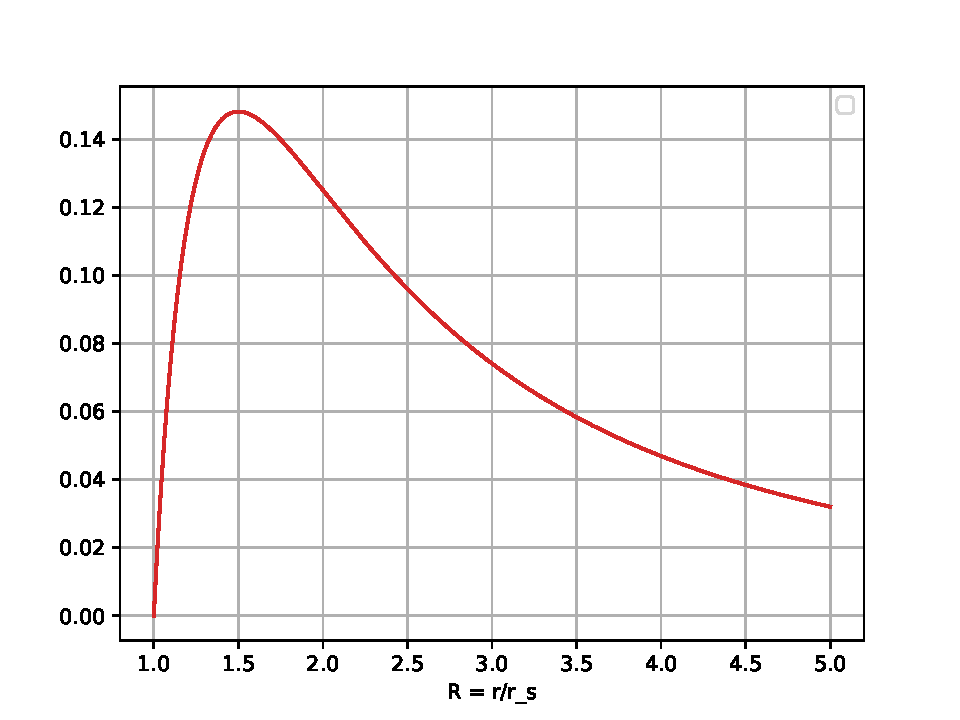
\includegraphics[width=0.7\textwidth]{figures/photon_effective_potential.pdf}
    \caption{Plot of the function \(R^{-2} - R^{-3}\).}
    \label{fig:effective-potential}
\end{figure}

The term \(b^{-2}\) is the maximum value which can be attained by the LHS: we can call it the total energy, the kinetic and potential contributions must add up to it. 
Also, the kinetic term is always positive. 
So, if the total energy is less than the maximum of the potential, the photon is constrained to stay on either side of the potential barrier around \(R = 3/2\). The potential there equals 
%
\begin{align}
  V(3/2) = (2GM)^{-2} \qty((3/2)^{-2} - (3/2)^{-3}) 
  = \frac{4/27}{(2GM)^2} = \frac{1}{27 (GM)^2}
\,,
\end{align} 
%
so the condition of the photon being above the potential barrier is 
%
\begin{align}
  E _{\text{tot}} &> V _{\text{max}}  \\
  \frac{e^2}{l^2} &> \frac{1}{27 G^2M^2}  \\
  \frac{l^2}{e ^2} &< 27G^2M^2
\,,
\end{align}
%
and under this condition, if the photon initially has positive \(\dv*{r}{\lambda }\) it will remain as such, since everything is continuous and (if the strict inequality is satisfied) we can never have \(\dv*{r}{\lambda }=0\). 

If instead we had \(l^2/e^2 < 27G^2M^2\) and the photon was initially travelling away from the black hole, there would come a point for which \(\dv*{r}{\lambda }\) would equal zero, and then it would become negative, since the photon could not go away from the center anymore. 

This can be understood graphically by drawing horizontal lines of constant total energy in the potential diagram. 

\subsubsection{A basis for a stationary observer}

If our observer's coordinates are \((t, r_{*}, \pi /2 , \varphi_{*} )\), that is, it is at rest with respect to our spatial coordinates but it is not following geodesic motion, then it will have nonzero 4-acceleration. So, since we know that velocity and acceleration are orthogonal, we can form our coordinate system as \((u^{\mu }, a^{\mu } / \sqrt{ a^{\rho } a_{\rho }}, e_{\theta }, e_{\varphi })\), where the angular basis vectors are simply normalized vectors in the \(\theta \) and \(\varphi \) directions.

This method has the advantage of being easily generalizable to find a comoving basis for any non-geodesic motion of our observer. 

Their 4-velocity must be normalized so that \(u^{\mu } u_{\mu }= -1\): so 
%
\begin{align}
  u^{\mu } = \left[\begin{array}{c}
  \dv{t}{\tau } \\ 
  0 \\ 
  0 \\ 
  0
  \end{array}\right]
  = 
  \left[\begin{array}{c}
  1/\sqrt{1 - \frac{2GM}{r}} \\ 
  0 \\ 
  0 \\ 
  0
  \end{array}\right]
\,,
\end{align}
%
then we can compute the 4-acceleration: it will be 
%
\begin{align}
  a^{\mu } &= u^{\nu } \nabla_{\nu } u^{\mu }
  = u^{\nu } \qty(\partial_{\nu } u^{\mu } + \Gamma^{\mu }_{\nu \rho } u^{\rho })  \\
  &= \frac{1}{\sqrt{1 - \frac{2GM}{r}}} \qty(\cancelto{}{\partial_{t} u^{\mu }} + \Gamma^{\mu }_{tt} u^{t})  \\
  &= \frac{1}{\sqrt{1-\frac{2GM}{r}}}
  \frac{1}{\sqrt{1-\frac{2GM}{r}}} \frac{A'}{2B} \delta^{\mu }_{r}
\,,
\end{align}
%
where \(A = 1/B = (1 - 2GM/r)\) are the coefficients of the Schwarzschild metric, with respect to which the Christoffel symbols are expressed in \eqref{eq:schwarzschild-christoffel}. 
The \(\delta^{\mu }_{r}\) signifies that the only component which survives is the radial one.
The two square root terms simplify the \(B\), so we get that the only nonzero component of the 4-acceleration is:
%
\begin{align}
  a^{r} = \frac{A^{\prime }}{2} =
  \frac{1}{2} \dv{}{r} \qty(1 - \frac{2GM}{r})
  = \frac{GM}{r^2}
\,.
\end{align}
%
The actual value of this component is not actually useful to us --- except as an illustration of the equivalence principle: it is the precise value of the Newtonian pseudo-force of acceleration --- since we need a normalized basis. Therefore, we will use a vector parallel to \(a^{\mu }\) but of length defined by the normalization \(e_{r} \cdot e_{r} = 1\). So, we get for our basis: 
%
\begin{align}
  \begin{cases}
    (e_{t})^{\mu } = u^{\mu } = \left[\begin{array}{cccc}
    (1-2GM/r)^{-1/2}, & 0, & 0, & 0
  \end{array}\right]^{\top} \\ 
    (e_{r})^{\mu } = a^{\mu } / \sqrt{a_{\rho } a^{\rho }}
  = \left[\begin{array}{cccc}
    0, & (1-2GM/r)^{1/2}, & 0, & 0
  \end{array}\right]^{\top}  \\
  (e_{\theta })^{\mu } = \left[\begin{array}{cccc}
  0, & 0, & 1/r, & 0
  \end{array}\right]^{\top} \\
  (e_{\varphi })^{\mu } = \left[\begin{array}{cccc}
  0, & 0, & 0, & 1/(r \sin \theta )
  \end{array}\right]^{\top}
\end{cases} 
\,,
\end{align}
%
where the last vector is written for a generic angle \(\theta \), but the sine is equal to one if \(\theta = \pi /2\). 
This basis satisfies the property \(e_{\alpha } \cdot e_{\beta } = \eta_{\alpha \beta }\). 

We will denote vectors written with respect to this basis with a subscript \(c\). 

\subsubsection{Critical angle of launch}

In the flat frame, the 4-velocity of the photon launched at \(\theta = \pi /2\) looks like: 
%
\begin{align}
  u^{\mu } _{\text{ph}} = \left[\begin{array}{c}
  1 \\ 
  \cos \psi  \\ 
  0 \\ 
  \sin \psi 
  \end{array}\right]_c
\,,
\end{align}
%
which means that in the Schwarzschild frame it looks like 
%
\begin{align}
  u^{\mu }_{\text{ph}} = \left[\begin{array}{c}
  \frac{1}{\sqrt{1-\frac{2GM}{r}}} \\ 
  \cos \psi \sqrt{1 - \frac{2GM}{r}} \\ 
  0 \\ 
  \frac{\sin \psi}{r} 
  \end{array}\right]
\,.
\end{align}

This means that the parameter \(l = r \sin \psi \), while \(e = \sqrt{1-2GM/r}\). 

The inequality to satisfy for the photon to be able to escape is: 
%
\begin{align}
  \qty[\frac{e^2}{l^2}]_{r_{*}} \geq \frac{1}{27G^2M^2}
\,,
\end{align}
%
which translates to 
%
\begin{align}
  \frac{1 - \frac{2GM}{r_{*}}}{r_{*}^2 \sin^2 \psi } \geq \frac{1}{27G^2M^2}
\,,
\end{align}
%
or 
%
\begin{align}
  r_{*}^2 \sin^2 \psi \leq 27G^2M^2 \qty(1 - 2GM/r_{*}) 
\,,
\end{align}
%
which once again can be expressed in terms of the adimensional radial coordinate \(R = r/2GM\): we find 
%
\begin{align}
  \sin^2 \psi \leq \frac{27}{4 R_{*}^2} \qty(1 - \frac{1}{R_{*}})
  \,,
\end{align}
%
so the critical angle can be computed by inverting this relation, which gives the plot shown in figure \ref{fig:critical-psi}.

\begin{figure}[ht]
  \centering
  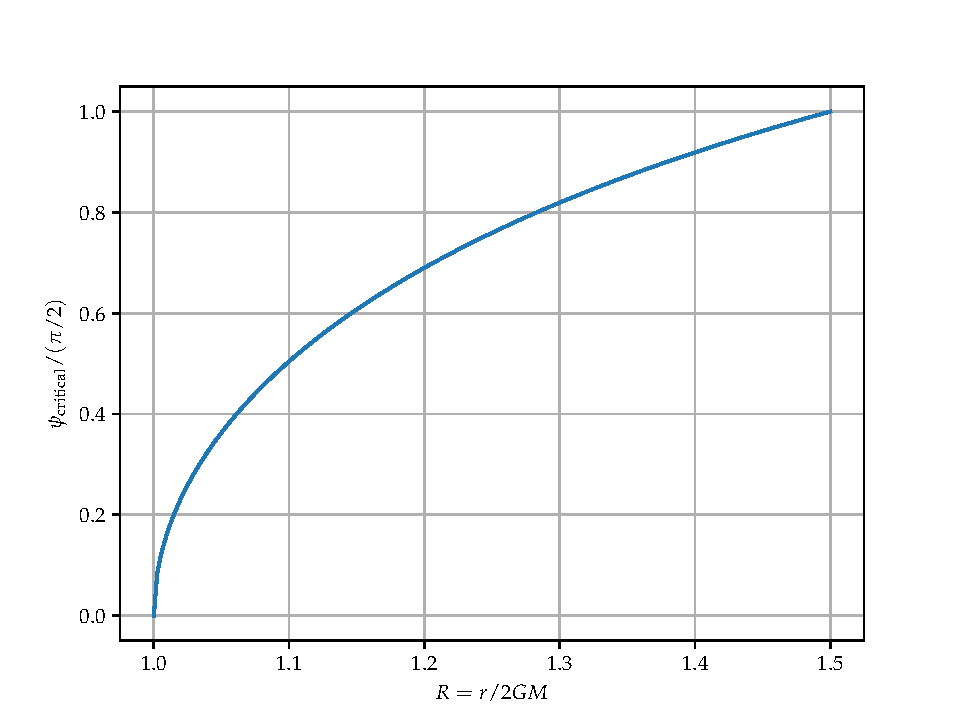
\includegraphics[width=0.7\textwidth]{figures/critical_psi.pdf}
  \caption{Critical angle}
  \label{fig:critical-psi}
\end{figure}
\end{document}